% Options for packages loaded elsewhere
\PassOptionsToPackage{unicode}{hyperref}
\PassOptionsToPackage{hyphens}{url}
%
\documentclass[
]{article}
\usepackage{amsmath,amssymb}
\usepackage{lmodern}
\usepackage{iftex}
\ifPDFTeX
  \usepackage[T1]{fontenc}
  \usepackage[utf8]{inputenc}
  \usepackage{textcomp} % provide euro and other symbols
\else % if luatex or xetex
  \usepackage{unicode-math}
  \defaultfontfeatures{Scale=MatchLowercase}
  \defaultfontfeatures[\rmfamily]{Ligatures=TeX,Scale=1}
\fi
% Use upquote if available, for straight quotes in verbatim environments
\IfFileExists{upquote.sty}{\usepackage{upquote}}{}
\IfFileExists{microtype.sty}{% use microtype if available
  \usepackage[]{microtype}
  \UseMicrotypeSet[protrusion]{basicmath} % disable protrusion for tt fonts
}{}
\makeatletter
\@ifundefined{KOMAClassName}{% if non-KOMA class
  \IfFileExists{parskip.sty}{%
    \usepackage{parskip}
  }{% else
    \setlength{\parindent}{0pt}
    \setlength{\parskip}{6pt plus 2pt minus 1pt}}
}{% if KOMA class
  \KOMAoptions{parskip=half}}
\makeatother
\usepackage{xcolor}
\usepackage[margin=1in]{geometry}
\usepackage{graphicx}
\makeatletter
\def\maxwidth{\ifdim\Gin@nat@width>\linewidth\linewidth\else\Gin@nat@width\fi}
\def\maxheight{\ifdim\Gin@nat@height>\textheight\textheight\else\Gin@nat@height\fi}
\makeatother
% Scale images if necessary, so that they will not overflow the page
% margins by default, and it is still possible to overwrite the defaults
% using explicit options in \includegraphics[width, height, ...]{}
\setkeys{Gin}{width=\maxwidth,height=\maxheight,keepaspectratio}
% Set default figure placement to htbp
\makeatletter
\def\fps@figure{htbp}
\makeatother
\setlength{\emergencystretch}{3em} % prevent overfull lines
\providecommand{\tightlist}{%
  \setlength{\itemsep}{0pt}\setlength{\parskip}{0pt}}
\setcounter{secnumdepth}{-\maxdimen} % remove section numbering
\ifLuaTeX
  \usepackage{selnolig}  % disable illegal ligatures
\fi
\IfFileExists{bookmark.sty}{\usepackage{bookmark}}{\usepackage{hyperref}}
\IfFileExists{xurl.sty}{\usepackage{xurl}}{} % add URL line breaks if available
\urlstyle{same} % disable monospaced font for URLs
\hypersetup{
  pdftitle={Yaquina Head Outstanding Natural Area Seabird Colony Monitoring 2023 Annual Report},
  pdfauthor={Will Kennerley},
  hidelinks,
  pdfcreator={LaTeX via pandoc}}

\title{Yaquina Head Outstanding Natural Area Seabird Colony Monitoring
2023 Annual Report}
\author{Will Kennerley}
\date{2023-09-05}

\begin{document}
\maketitle

Yaquina Head Seabird Colony Yaquina Head Outstanding Natural Area,
Newport, Oregon 2022 Season Summary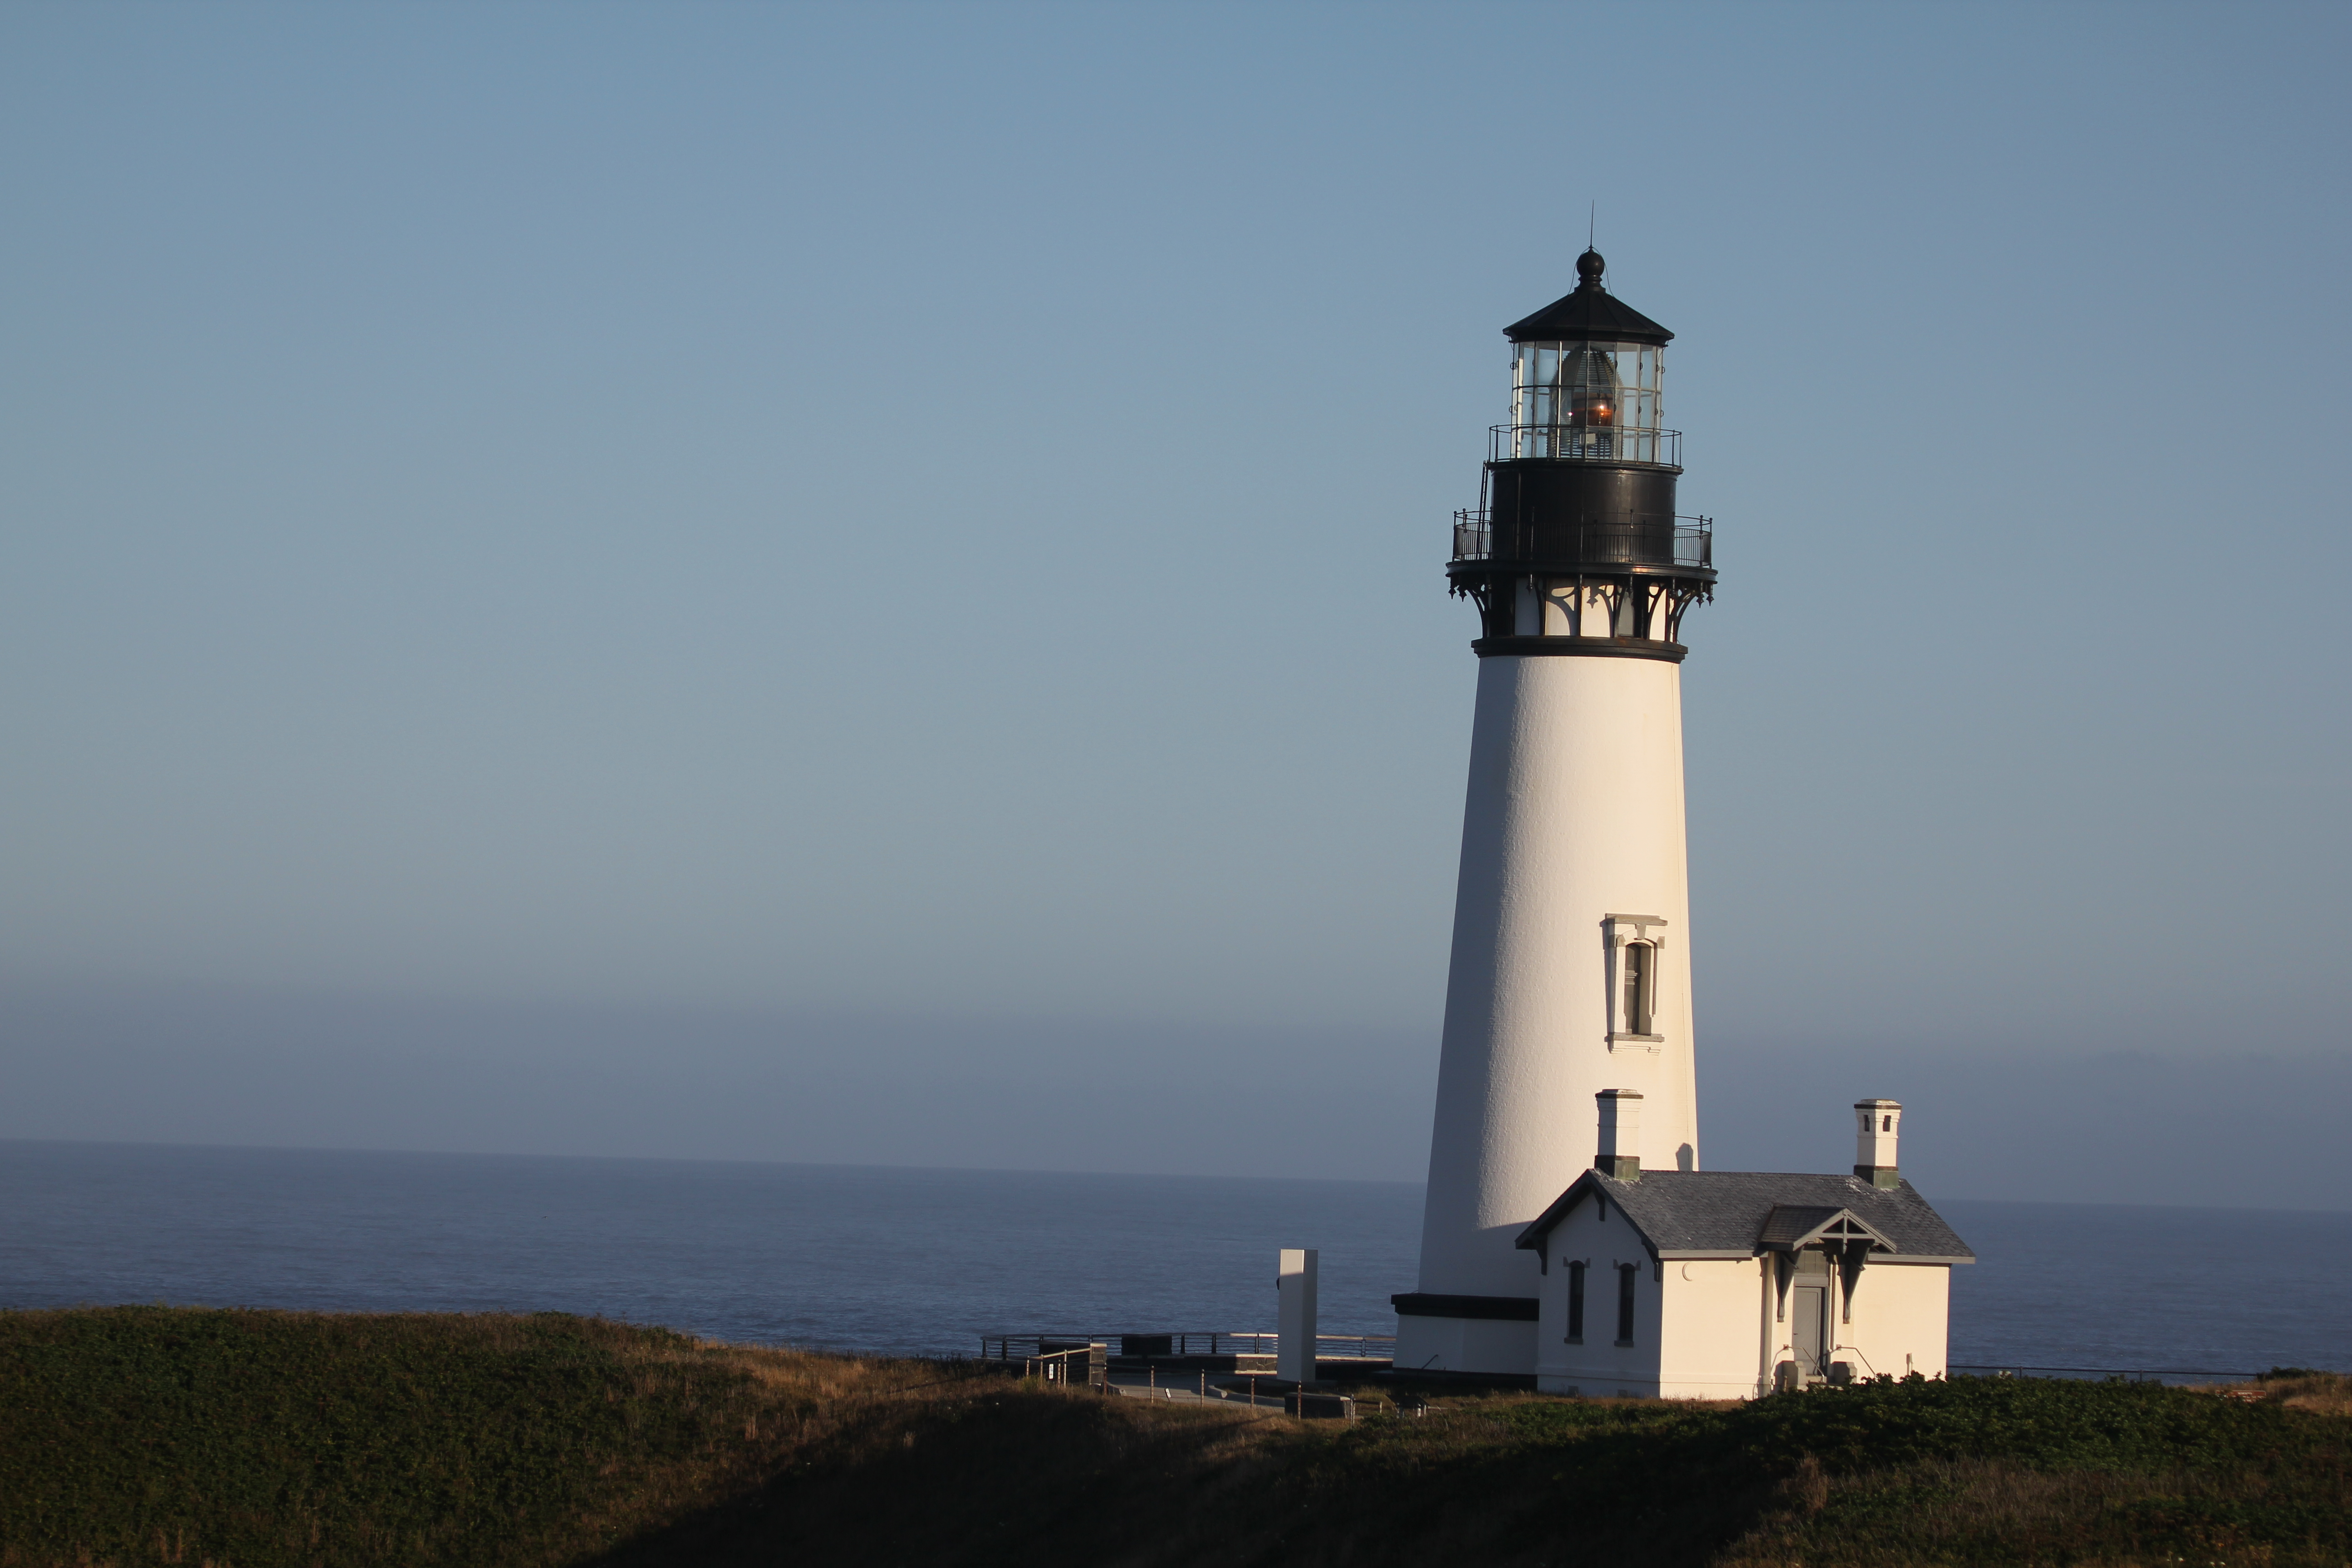
\includegraphics{images/IMG_1692.JPG}

Will Kennerley \& Rachael Orben Seabird Oceanography Lab, Oregon State
University

Project Overview

Yaquina Head Outstanding Natural Area (YHONA) is home to some of
Oregon's largest

and most publicly visible seabird colonies, and has included over 60,000
Common Murres ( Uria

aalge ) in peak attendance years. The seabird colonies surrounding
Yaquina Head present a

unique opportunity for research and monitoring given their close
proximity to viewing platforms

and intensive oceanographic studies of surrounding waters. From 1980 to
2010 the common

murre population at Yaquina Head experienced rapid growth and
reproductive success however,

there has been significant fluctuation and reproductive failures over
the last 8-10 years. The 2022

field season was the 16 th consecutive year of murre productivity
monitoring; a collaborative

effort between Oregon State University, U.S. Fish and Wildlife Service,
and the Bureau of Land

Management. In combination with similar studies conducted by Julia
Parrish of the University of

Washington from 1998 -- 2002, our investigation of seabirds at Yaquina
Head has contributed to

a 21-year time series of observation.

In general, we are interested in how seabird breeding chronology,
reproductive success,

diet, and foraging activities are affected by changing ocean conditions.
However, another

important dynamic occurring at Yaquina Head is murre depredation
coincident with increasing

bald eagle ( Haliaeetus leucocephalus ) interactions. Our study
objectives include quantifying the

effects of bald eagles and other sources of predation on or disturbance
to seabirds during the

breeding season.

Observations were conducted from the public viewing deck at the base of
the lighthouse.

Construction modified the viewing deck slightly from previous years
making the viewing

platform slightly lower. Plots were monitored from May through August
three to four days per

week (about every other day). Common murre nest checks began in late
May, however nesting

attempts were repeatedly disturbed and rocks were frequently abandoned
upon arrival. Murres

failed to successfully establish nests in 2022, leading to a total
breeding failure for common

murres at Yaquina Head. Eggs at nest sites were spotted frequently early
in the breeding season,

but egg depredation was observed within the same day of each confirmed
egg sighting in all

cases. In years more successful breeding, we closely observed breeding
birds, documented when

eggs were laid and then monitored the progressive success of the
breeding pairs through egg

incubation and chick rearing. We observed disturbances to the breeding
colony and recorded the

frequency, duration and consequences (e.g., loss of eggs or chicks) of
these events during our

\end{document}
